%-----------------------------------------------------------------
%	QUANTUM LIGHT-MATTER INTERACTION
%	!TEX root = ./../main.tex
%-----------------------------------------------------------------
\section{Quantum light--matter interaction}
\subsection{Jaynes--Cummings model}
Let's consider a two-level atom (figure \ref{fig:two-level-cummings}) and only one mode of the field.
\begin{figure}[H]
	\centering
	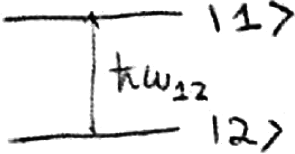
\includegraphics[width=0.2\textwidth]{./images/5-two-level-cummings}
	\caption{A two-level atom, where $\ket{2}$ is the ground state}
	\label{fig:two-level-cummings}
\end{figure}

In this system, an arbitrary state, $\ket{\psi}$ can be written as
\begin{align}
	\ket{\psi} = c_{1} \ket{1} + c_{2} \ket{2} = \mqty(c_{1} \\ c_{2})
\end{align}

\begin{defi}[Pauli matrices]
	\begin{align}
		\hat{\sigma}_{x} = \mqty(\pmat{1}) \qc \hat{\sigma}_{y} = \mqty(\pmat{2}) \qc \hat{\sigma}_{z} = \mqty(\pmat{3})
	\end{align}
\end{defi}

\begin{defi}[Lowering and rising operators]
	\begin{align}
		\hat{\sigma}_{+} = \frac{1}{2} (\hat{\sigma}_{x} + i \hat{\sigma}_{y}) = \mqty(0 & 1 \\ 0 & 0) \qc \hat{\sigma}_{-} = \frac{1}{2} (\hat{\sigma}_{x} - i \hat{\sigma}_{y}) = \mqty(0 & 0 \\ 1 & 0)
	\end{align}
	Therefore, in a two-level system, the lowering and rising operators act upon the atomic level:
	\begin{align*}
		\hat{\sigma}_{+} \ket{2} = \ket{1} \qc \hat{\sigma}_{-} \ket{1} = \ket{2}
	\end{align*}
\end{defi}

Let's work out the Hamiltonian, $\hat{H} = \hat{H}_{a} + \trn{\hat{H}} + \hat{V}$:
\begin{align}
	\hat{H}_{a} = \frac{\hbar}{2} \omega_{12} \hat{\sigma}_{z} \qc \trn{\hat{H}} = \hbar \omega \hat{a}\sdag \hat{a} \qc \hat{V} = - \hat{\va{\mu}} \vdot \trn{\hat{\va{E}}}
\end{align}
For the atomic Hamiltonian, $\hat{H}_{a}$, we've fixed the the origin of energy in the middle of $\ket{1}$ and $\ket{2}$. Now we need to develop the interaction Hamiltonian:
\begin{flalign*}
	\hat{V} &= - \hat{\va{\mu}} \vdot \trn{\hat{\va{E}}} = - \mu_{0} \trn{\hat{E}} (\hat{\sigma}_{-} + \hat{\sigma}_{+}) \overset{\text{EDA}}{\Longrightarrow} \trn{\hat{E}} = i \mc{E}_{\omega} (\hat{a} - \hat{a}\sdag) \Rightarrow \hat{V} = - i g \hbar (\hat{a} - \hat{a}\sdag) (\hat{\sigma}_{-} + \hat{\sigma}_{+}) & \\
	&= - ig \hbar (\underbrace{\hat{a} \hat{\sigma}_{-}}_{\text{(a)}} + \underbrace{\hat{a} \hat{\sigma}_{+}}_{\text{(b)}} - \underbrace{\hat{a}\sdag \hat{\sigma}_{-}}_{\text{(c)}} - \underbrace{\hat{a}\sdag \hat{\sigma}_{+}}_{\text{(d)}})
\end{flalign*}
\begin{figure}[H]
	\centering
	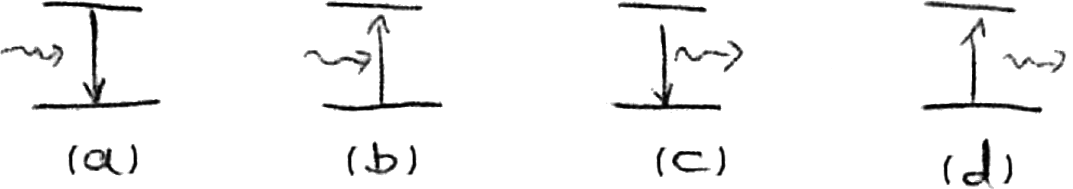
\includegraphics[width=0.6\textwidth]{./images/5-transitions}
	\caption{Possible atomic transitions: (b) is absorption, (c) is spontaneous emission, (a) and (d) are transitions that are only possible if they are fast enough}
	\label{fig:transitions}
\end{figure}
The pairs of operators have the following time dependence\footnote{We are considering the free evolution of the operators ($g = 0$).} in the Heisenberg picture:
\begin{subequations}
\begin{align}
	\hat{a}(t) \hat{\sigma}_{-}(t) &= \hat{a}(0) \hat{\sigma}_{-}(0) e^{-i(\omega + \omega_{0})t} \label{eq:asigma1} \\
	\hat{a}\sdag(t) \hat{\sigma}_{+}(t) &= \hat{a}\sdag(0) \hat{\sigma}_{+}(0) e^{i(\omega + \omega_{0})t} \label{eq:asigma2} \\
	\hat{a}(t) \hat{\sigma}_{+}(t) &= \hat{a}(0) \hat{\sigma}_{+}(0) e^{-i(\omega - \omega_{0})t} \label{eq:asigma3} \\
	\hat{a}\sdag(t) \hat{\sigma}_{-}(t) &= \hat{a}(\sdag0) \hat{\sigma}_{-}(0) e^{i(\omega - \omega_{0})t} \label{eq:asigma4}
\end{align}
\end{subequations}
The two first pairs (\ref{eq:asigma1},~\ref{eq:asigma2}) evolve at optical frequencies, which (near resonance) tend to average to zero in the course of a few optical periods compared to the pairs (\ref{eq:asigma3},~\ref{eq:asigma4}). This amounts to the same physics and mathematics that we used in discussing the RWA. Therefore, we get
\begin{align}
	\hat{V} = - ig \hbar (\hat{a} \hat{\sigma}_{+} - \hat{a}\sdag \hat{\sigma}_{-} )
\end{align}
where $g$ is the quantised Rabi frequency.

\begin{defi}[Quantised of the Rabi frequency]
	\begin{align}
		g \equiv \frac{\mu_{0} \mc{E}_{\omega}}{\hbar}
	\end{align}
\end{defi}

It's easy to prove in the Heisenberg picture that the full Hamiltonian in the Jaynes--Cunnings model is
\begin{align}
	\hat{H} = \underbrace{ \frac{\hbar}{2} \omega_{12} \hat{\sigma}_{z} + \hbar \omega \hat{a}\sdag \hat{a} }_{\hat{H}_{0}} - ig \hbar (\hat{a} \hat{\sigma}_{+} - \hat{a}\sdag \hat{\sigma}_{-} )
\end{align}

%-----------------------------------------------------------------
\subsection{Dressed atom}
\subsubsection*{Eigenstates}
The states $\ket{1, n}$ and $\ket{2, n}$ are eigenstates of the free Hamiltonian, $\hat{H}_{0}$, but the interaction Hamiltonian, $\hat{V}$, couples pairs of states (multiplets; $\xi_{n} = \qty{\ket{2, n+1}, \ket{1, n}}$) from the infinite set of eigenstates of the free Hamiltonian:
\begin{alignat*}{2}
	\hat{H}_{0} \ket{1, n} &= \qty(\frac{\hbar}{2} \omega_{12} + n \hbar \omega ) \ket{1, n} \qc & \hat{H}_{0} \ket{2, n+1} &= \qty(-\frac{\hbar}{2} \omega_{12} + (n+1) \hbar \omega ) \ket{2, n+1} \\
	\hat{V} \ket{1, n} &\mapsto \ket{2, n+1} \qc & \hat{V} \ket{2, n+1} &\mapsto \ket{1, n}
\end{alignat*}

Therefore, we can rewrite the full Hamiltonian as the sum of the Hamiltonians applied to each multiplet: $\hat{H} = \sum_{n} \hat{H}_{n}$, where the Hamiltonian applied to the multiplet $\xi_{n}$ is
\begin{align}
	\hat{H}_{n} = \hbar \qty(n + \frac{1}{2}) \omega \mqty(1 & 0 \\ 0 & 1) + \frac{\hbar}{2} \mqty( \Delta & - 2 i g \sqrt{n+1} \\ 2 i g \sqrt{n+1} & \Delta )
\end{align}
% WIP: Myestre says \mqty( \Delta & 2 g \sqrt{n+1} \\ 2 g \sqrt{n+1} & -\Delta )

\subsubsection*{Dressed states}
The dressed states of the two-level atom in the Jaynes--Cunnings model are
\begin{subequations}
\begin{align}
	\ket{-,n} &= \cos \theta_{n} \ket{1,n} - \sin \theta_{n} \ket{2,n+1} \\
	\ket{+,n} &= \sin \theta_{n} \ket{1,n} + \cos \theta_{n} \ket{2,n+1}
\end{align}
\end{subequations}
where $\Omega_{n}$ is the generalised quantised Rabi frequency, and $\theta_{n}$ are defined by
\begin{align*}
	\cos \theta_{n} = \frac{\Omega_{n} - \Delta}{\sqrt{(\Omega_{n} - \Delta)^{2} + 4 g^{2} (n+1)}} \qc \sin \theta_{n} = \frac{2 g \sqrt{n+1}}{\sqrt{(\Omega_{n} - \Delta)^{2} + 4 g^{2} (n+1)}}
\end{align*}

\begin{defi}[Generalised quantised Rabi frequency]
	\begin{align}
		\Omega_{n} \equiv \sqrt{\Delta^{2} + 4 g^{2} (n+1)}
	\end{align}
\end{defi}

The energies of the dressed states are
\begin{align}
	E_{n}^{\pm} = \hbar \qty(n + \frac{1}{2}) \omega \pm \frac{1}{2} \hbar \Omega_{n}
\end{align}

\begin{figure}[H]
	\centering
	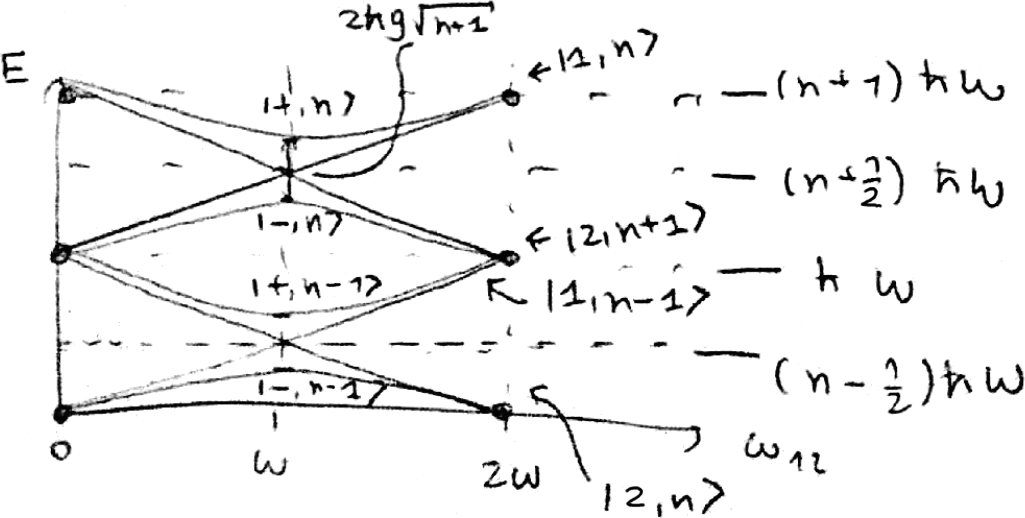
\includegraphics[width=0.7\textwidth]{./images/5-jc-energies}
	\caption{Energies of the dressed states under the Jaynes--Cunnings model}
	\label{fig:jc-energies}
\end{figure}

\subsubsection*{Mollow triplet}
In the Jaynes--Cunnings model, the photon emitted by spontaneous emission is not in the same mode of the Hamiltonian we are studying. Therefore, the atomic transition is between $\ket{1, n} \mapsto \ket{2, n}$. From the expressions of the dressed states we know that $\ket{1, n}$ is a linear combination of $\ket{+, n}$ and $\ket{-, n}$, whilst $\ket{2, n}$ is a linear combination of $\ket{+, n-1}$ and $\ket{-, n-1}$. Therefore, assuming that $\Omega_{n} \sim \Omega_{n+1}$ for a sufficiently large $n$, the transitions in the dressed basis are the following:
\begin{itemize}
	\item $\ket{-, n} \mapsto \ket{-, n-1} \Rightarrow E = \hbar \omega$.
	\item $\ket{-, n} \mapsto \ket{+, n-1} \Rightarrow E = \hbar (\omega - \Omega_{n})$.
	\item $\ket{+, n} \mapsto \ket{-, n-1} \Rightarrow E = \hbar (\omega + \Omega_{n})$.
	\item $\ket{+, n} \mapsto \ket{+, n-1} \Rightarrow E = \hbar \omega$.
\end{itemize}

\begin{figure}[H]
	\centering
	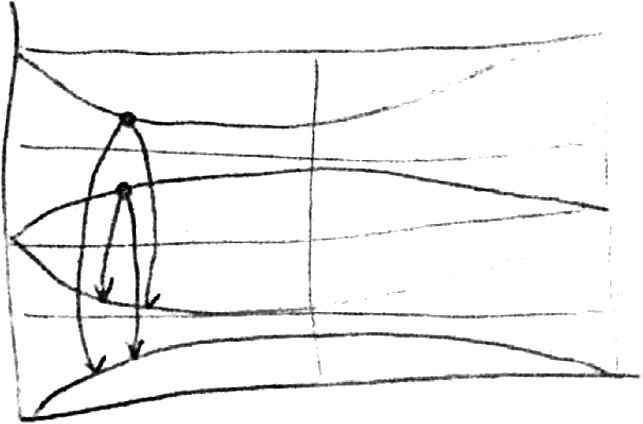
\includegraphics[width=0.5\textwidth]{./images/5-jc-mollow-triplet}
	\caption{Mollow triplet under the Jaynes--Cunnings model}
	\label{fig:jc-mollow-triplet}
\end{figure}

\subsubsection*{Autner--Townes doublet}
% WIP: expand from the exercises
\begin{figure}[H]
	\centering
	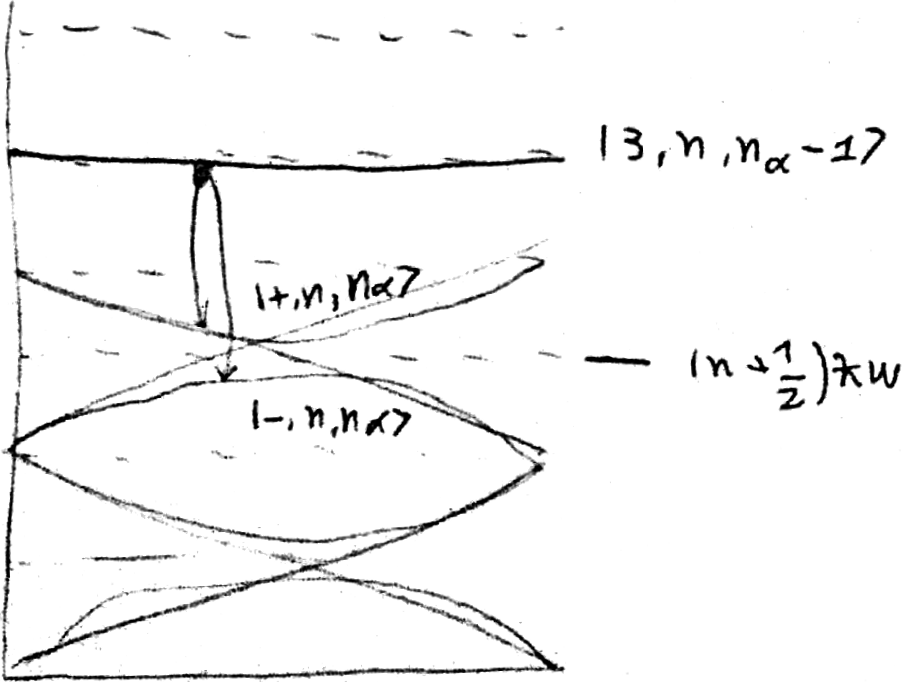
\includegraphics[width=0.55\textwidth]{./images/5-jc-autler-townes-doublet}
	\caption{Autner--Townes doublet under the Jaynes--Cunnings model}
	\label{fig:jc-autler-townes-doublet}
\end{figure}

%-----------------------------------------------------------------
\subsection{Quantum Rabi oscillations}
Since the dressed states, $\ket{\pm, n}$, are the eigenstates of the full Hamiltonian, we can use the integral form of the Schrödinger equation to calculate the temporal evolution of an arbitrary state, $\ket{\psi (t)}$:
\begin{flalign*}
	\ket{\psi(t)} &= \exp\qty{- i \frac{\hat{H}}{\hbar} t} \ket{\psi(0)} = \sum_{n=0}^{\infty} \sum_{j=\pm} \exp{-i \frac{E_{n}^{j}}{\hbar} t} \ket{j,n} \braket{j,n}{\psi(0)} & \\
	&\Rightarrow \mqty(c_{-,n}(t) \\ c_{+,n}(t)) = \mqty(\exp{i \frac{\Omega_{n}}{2} t} & 0 \\ 0 & \exp{-i \frac{\Omega_{n}}{2} t} ) \mqty(c_{-,n}(0) \\ c_{+,n}(0))
\end{flalign*}
The dressed basis can be interpreted as a transformation of the bare basis:
\begin{align}
	\mqty(c_{-,n}(t) \\ c_{+,n}(t)) = T \mqty(c_{1,n}(t) \\ c_{2,n+1}(t)) \qc T = \mqty( \cos \theta_{n} & - \sin \theta_{n} \\ \sin \theta_{n} & \cos \theta_{n})
\end{align}

Therefore, we can find the temporal evolution of the bare basis, which can be simplified further applying the RWA:
\begin{flalign*}
	\mqty(c_{1,n}(t) \\ c_{2,n+1}(t)) &= T^{-1} \mqty(\exp{i \frac{\Omega_{n}}{2} t} & 0 \\ 0 & \exp{-i \frac{\Omega_{n}}{2} t} ) T \mqty(c_{1,n}(0) \\ c_{2,n+1}(0)) & \\
	&= \mqty( \cos(\dfrac{\Omega_{n}}{2} t) - i \dfrac{\Delta}{\Omega_{n}} \sin(\dfrac{\Omega_{n}}{2} t) & - i \dfrac{2 g}{\Omega_{n}} \sqrt{n+1} \sin(\dfrac{\Omega_{n}}{2} t) \\ - i \dfrac{2 g}{\Omega_{n}} \sqrt{n+1} \sin(\dfrac{\Omega_{n}}{2} t) & \cos(\dfrac{\Omega_{n}}{2} t) + i \dfrac{\Delta}{\Omega_{n}} \sin(\dfrac{\Omega_{n}}{2} t) ) \mqty(c_{1,n}(0) \\ c_{2,n+1}(0))
\end{flalign*}

With the initial conditions $c_{1,n}(0) \equiv 1$ and $c_{2,n}(0) \equiv 0$, it's easy to see that
\begin{align}
	\mqty(c_{1,n}(t) \\ c_{2,n+1}(t)) = \mqty( \cos(\dfrac{\Omega_{n}}{2} t) - i \dfrac{\Delta}{\Omega_{n}} \sin(\dfrac{\Omega_{n}}{2} t) \\ - i \dfrac{2 g}{\Omega_{n}} \sqrt{n+1} \sin(\dfrac{\Omega_{n}}{2} t) )
\end{align}

\subsubsection*{Populations}
Since the expressions for $c_{1,n}(t)$ and $c_{2,n+1}(t)$ are relatively simple, we can calculate the temporal evolution of the populations:
\begin{subequations}
\begin{align}
	P_{1,n} (t) &= \norm{c_{1,n}(t)}^{2} = \cos[2](\frac{\Omega_{n}}{2} t) + \frac{\Delta^{2}}{\Omega_{n}^{2}} \sin[2](\frac{\Omega_{n}}{2} t) \\
	P_{2,n+1} (t) &= \norm{c_{2,n+1}(t)}^{2} = \frac{4 g^{2} (n+1)}{\Omega_{n}^{2}} \sin[2](\frac{\Omega_{n}}{2} t)
\end{align}
\end{subequations}

In resonance ($\Delta = 0$), these expressions are much simpler:
\begin{align}
	P_{1,n} (t) = \cos[2](g \sqrt{n+1} \, t) \qc P_{2,n+1} (t) = \sin[2](g \sqrt{n+1} \, t)
\end{align}

This $\Omega_{n}$ Rabi frequency is special, because it depends on $n+1$. This means the vacuum has Rabi oscillations as well.
%-----------------------------------------------------------------
\subsection{Collapses and revivals}
If we illuminate the atom with a coherent state, $\ket{\alpha}$, instead of a Fock state, $\ket{n}$, then the population becomes a superposition of oscillations: $P_{1, \alpha} = \sum_{n} P(n) \norm{c_{1,n}(t)}^{2}$. In resonance we have
\begin{align}
	P_{1,\alpha} = e^{-\abs{\alpha}^{2}} \sum_{n} \frac{\abs{\alpha}^{2n}}{n!} \cos[2](g \sqrt{n+1} \, t)
\end{align}

Since we have a superposition of oscillations, the population decays because of the dephasing (collapse). However, the superposition is a discrete sum, so after a certain time, the oscillations start to be in phase again (revival).
\begin{figure}[H]
	\centering
	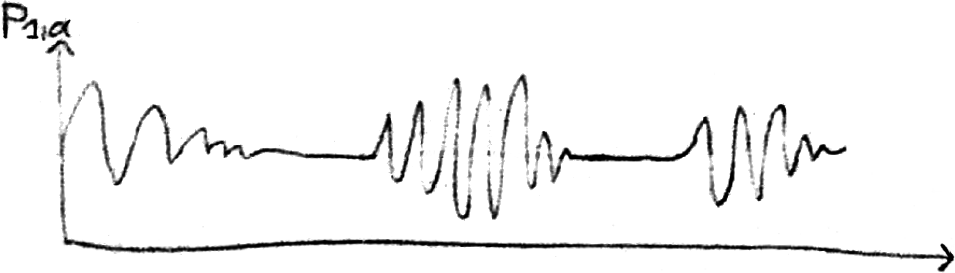
\includegraphics[width=0.7\textwidth]{./images/5-collapses-revivals}
	\caption{Collapses and revivals of the population}
	\label{fig:collapses-revivals}
\end{figure}
The collapse and revival times are given by
\begin{align}
	t_{c}(\Omega_{\ev{n} - \Delta n} - \Omega_{\ev{n} + \Delta n} ) \sim 1 \qc t_{r}(\Omega_{\ev{n}} - \Omega_{\ev{n} -1} ) \sim 2\pi m \qc m \in \mbb{N}
\end{align}

%-----------------------------------------------------------------
\subsection{Weisskopf--Wigner theory of spontaneous emission}
Armed with a proper three-dimensional density matrix formalism and the quantum light description, we can study the spontaneous emission of an excited state atom into the electromagnetic vacuum.
\begin{figure}[H]
	\centering
	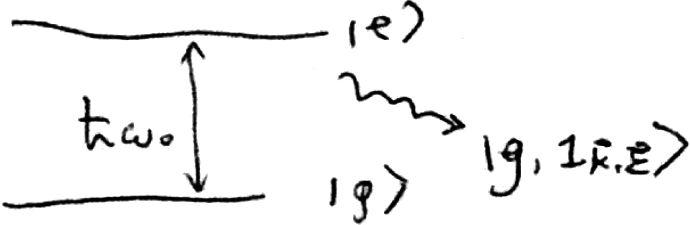
\includegraphics[width=0.4\textwidth]{./images/5-two-level-weisskopf}
	\caption{Spontaneous emission in a two level atom}
	\label{figtwo-level-weisskopf:}
\end{figure}

Let's work out the Hamiltonian, $\hat{H} = \hat{H}_{a} + \trn{\hat{H}} + \hat{V}$:
\begin{align}
	\hat{H}_{a} = \hbar \omega_{0} \dyad{e} \qc \trn{\hat{H}} = \sum_{\va{k},\vu{\epsilon}} \hbar \omega_{k} \qty(n_{\va{k},\vu{\epsilon}} + \frac{1}{2}) \qc \hat{V} = \sum_{\va{k},\vu{\epsilon}} \qty(\hbar g_{\va{k},\vu{\epsilon}} \hat{a}_{\va{k},\vu{\epsilon}} \hat{\sigma}_{+} + \Hc )
\end{align}
where $\hat{\mu} = \va{\mu}_{0} (\hat{\sigma}_{+} + \hat{\sigma}_{-})$, $\dsp \hat{E} = \sum_{\va{k},\vu{\epsilon}} i\qty(\mc{E}_{c} \vu{\epsilon}_{k} \hat{a}_{\va{k},\vu{\epsilon}} - \Hc )$, and $\dsp g_{\va{k},\vu{\epsilon}} = i \sqrt{\frac{\omega_{k}}{2 \hbar \varepsilon_{0} L^{3} }} \va{\mu}_{0} \vu{\epsilon}_{\va{k}}$.

Fixing the initial condition to $\ket{\psi (0)} = \ket{e, \qty{0}}$ reduces the general state vector to
\begin{align}
	\ket{\psi (t)} = c(t) e^{-i \omega_{0} t} \ket{e,\qty{0}} + \sum_{\va{k},\vu{\epsilon}} b_{\va{k},\vu{\epsilon}} (t) e^{-i \omega_{k} t} \ket{g, 1_{\va{k},\vu{\epsilon}}}
\end{align}
where $c(t)$ and $b_{\va{k},\vu{\epsilon}}(t)$ are, respectively, the probability amplitudes of the excited and ground states.

From the Schrödinger equation, $\dsp \hat{H} \ket{\psi (t)} = i \hbar \dv{\ket{\psi (t)}}{t}$, we can calculate the temporal evolution of the probability amplitudes:
\begin{subequations}
\begin{align}
	\dot{c}(t) &= i \sum_{\va{k},\vu{\epsilon}} g_{\va{k},\vu{\epsilon}} e^{-i (\omega_{k} - \omega_{0}) t} b_{\va{k},\vu{\epsilon}} (t) \\
	\dot{b}_{\va{k},\vu{\epsilon}}(t) &= i g_{\va{k},\vu{\epsilon}}\sast e^{i (\omega_{k} - \omega_{0}) t} c(t)
\end{align}
\end{subequations}
Let's work out the solution of $c(t)$:
\begin{flalign*}
	b_{\va{k},\vu{\epsilon}}(t) &= i g_{\va{k},\vu{\epsilon}}\sast \int_{0}^{t} e^{i (\omega_{k} - \omega_{0}) t'} c(t') \dd{t'} \Rightarrow \dot{c}(t) = - \sum_{\va{k},\vu{\epsilon}} \norm*{g_{\va{k},\vu{\epsilon}}}^{2} \int_{0}^{t} e^{-i(\omega_{k} - \omega_{0})(t - t')} c(t') \dd{t'} &
\end{flalign*}
Now we need to calculate the sum of $\norm*{g_{\va{k},\vu{\epsilon}}}^{2}$:
\begin{flalign*}
	\sum_{\va{k},\vu{\epsilon}} \norm*{g_{\va{k},\vu{\epsilon}}}^{2} &= \sum_{\va{k},\vu{\epsilon}} \frac{\omega_{k}}{2 \hbar \varepsilon_{0} L^{3}} (\va{\mu}_{0} \vdot \vu{\epsilon}_{\va{k}})^{2} \underset{L \to \infty}{\longrightarrow} \int \dd[3]{k} \sum_{\vu{\epsilon}} \frac{\omega_{k}}{2 \hbar \varepsilon_{0} (2 \pi)^{3}} (\va{\mu}_{0} \vdot \vu{\epsilon}(\va{k}))^{2} &\\
	&= \int_{0}^{\infty} \dd{k} k^{2} \frac{\omega_{k}}{2 \hbar \varepsilon_{0} (2 \pi)^{3}} \qty{ \sum_{j = 1}^{2} \int_{0}^{\pi} \sin \theta \dd{\theta} \int_{0}^{2\pi} \dd{\phi} (\va{\mu}_{0} \vdot \vu{\epsilon}_{j}(\va{k}))^{2} }
\end{flalign*}
Since $\qty{\vu{\epsilon}_{1}, \vu{\epsilon}_{2}, \va{k}}$ form an orthonormal basis, we can write any vector in that basis. In particular, we can write $\norm*{\va{\mu}_{0}}^{2} = (\va{\mu}_{0} \vdot \vu{\epsilon}_{1})^{2} + (\va{\mu}_{0} \vdot \vu{\epsilon}_{2})^{2} + (\va{\mu}_{0} \vdot \va{k})^{2}$. Geometrically, $(\va{\mu}_{0} \vdot \va{k})^{2} = \norm*{\va{\mu}_{0}}^{2} \cos^{2} \theta$; consequently, $\sum_{i = 1}^{2} (\va{\mu}_{0} \vdot \vu{\epsilon}_{i}(\va{k}))^{2} = \norm*{\va{\mu}_{0}}^{2} \sin^{2} \theta$. Therefore,
\begin{flalign*}
	\sum_{\va{k},\vu{\epsilon}} \norm*{g_{\va{k},\vu{\epsilon}}}^{2} &= \int_{0}^{\infty} \dd{k} k^{2} \frac{\omega_{k}}{2 \hbar \varepsilon_{0} (2 \pi)^{3}} \int_{0}^{\pi} \sin^{3} \theta \dd{\theta} \int_{0}^{2\pi} \dd{\phi} \norm*{\va{\mu}_{0}}^{2} = \frac{\norm*{\va{\mu}_{0}}^{2}}{6 \pi^{2} \varepsilon_{0} \hbar c^{3}} \int_{0}^{\infty} \omega_{k}^{3} \dd{\omega_{k}}. &
\end{flalign*}
Now that we have found an expression for $\sum_{\va{k},\vu{\epsilon}} \norm*{g_{\va{k},\vu{\epsilon}}}^{2}$, we can find a simpler expression for $\dot{c}(t)$. Since $\omega_{k} \sim \omega_{0}$, $e^{-i(\omega_{k} - \omega_{0})} \approx 1$, meaning that $\int \dd{\omega_{k}} e^{-i(\omega_{k} - \omega_{0})(t - t')} \approx 2 \pi \delta(t-t')$; this also means that the photon emitted by spontaneous emission will have the natural frequency of the two-level atom, $\omega_{0}$. Therfore,
\begin{flalign*}
	\dot{c}(t) &= - \frac{\norm*{\va{\mu}_{0}}^{2}}{6 \pi^{2} \varepsilon_{0} \hbar c^{3}} \int_{0}^{\infty} \omega_{k}^{3} \dd{\omega_{k}} \int_{0}^{t} e^{-i(\omega_{k} - \omega_{0})(t - t')} c(t') \dd{t'} & \\
	&\approx - \frac{\norm*{\va{\mu}_{0}}^{2}}{6 \pi^{2} \varepsilon_{0} \hbar c^{3}} \omega_{0}^{3} \int_{0}^{t} 2\pi \delta(t - t') c(t') \dd{t'} = - \frac{\norm*{\va{\mu}_{0}}^{2} \omega_{0}^{3}}{3 \pi \varepsilon_{0} \hbar c^{3}} c(t) \equiv - \Gamma c(t)
\end{flalign*}
Therefore, the temporal evolution of the probability amplitude of the excited state follows an exponential decay:
\begin{align}
	c(t) = e^{- \Gamma t} c(0) \qc \Gamma = \frac{\norm*{\va{\mu}_{0}}^{2} \omega_{0}^{3}}{3 \pi \varepsilon_{0} \hbar c^{3}}
\end{align}

Knowing the expression of $c(t)$, it's not difficult to see that, for $t \to \infty$, the probability amplitude of the ground state follows a Lorentzian:
\begin{align}
	\lim_{t \to \infty} \norm*{b_{\va{k}, \vu{\epsilon}}}^{2} = \frac{\norm*{g_{\va{k}, \vu{\epsilon}}}^{2}}{\Gamma^{2} + (\omega_{k} - \omega_{0})^{2}}
\end{align}

%-----------------------------------------------------------------
\subsection{Cavity quantum electrodynamics}
By using Rydberg atoms and a high-$Q$ cavity, one can realise the Jaynes--Cunnings model and treat the system as two-level atom and one mode of the electromagnetic field.

The reasons and advantages of using Rydberg atoms are:
\begin{itemize}
	\item Circular Rydberg atoms have a very large $n$ energy level (in Serge Haroche's experiments, $n \sim 50$).
	\item Only one electric dipole transition is allowed, which is very close to a two-level atom transition.
	\item They have very large classical radius ($r \sim n^{2} a_{0}$), therefore $\mu_{0} = \mel{n}{\mu}{n'} \sim e n^{2} a_{0}$.
	\item The decay rate is $\Gamma \propto \omega^{3}$. Since the transitions are in the microwave regime, the Rydberg atoms have a very long lifetime.
	\item They are easily ionisable, which is useful for the detection of the properties of the system.
\end{itemize}
